\documentclass[aspectratio=43]{beamer}
%Information to be included in the title page:
\title{Paper Reading}
\author{Dachun Kai}
\institute{USTC}
\date{December 17, 2021}
%\usetheme{CambridgeUS}
\usetheme{Boadilla}

\usepackage[backend=bibtex,sorting=none]{biblatex}
%\usepackage{ctex}
\addbibresource{ref.bib} %BibTeX数据文件及位置
\setbeamerfont{footnote}{size=\tiny}
\usepackage{graphicx}
\usepackage{animate}
\usepackage{hyperref}
\usepackage{caption}
\usepackage{extarrows}

\begin{document}
	\frame{\titlepage}
	
	\begin{frame}{WEVI\textit{(ICCV2021)}}
		\begin{figure}
			\centering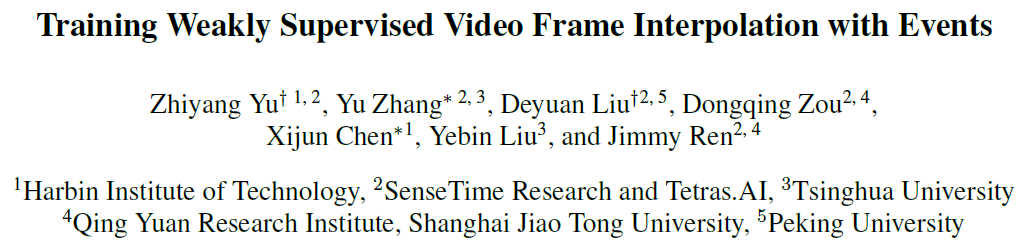
\includegraphics[width=0.75\linewidth]{images/title.png}
		\end{figure}
	\end{frame}
	
	\begin{frame}{Preliminaries}
	\only<1>{
		\framesubtitle{{\normalsize Weakly Supervised learning}}
		\begin{itemize}
			\item {\large Incomplete supervision: subset labels} $ \to $ \alert{trained on low frame-rate videos} \\
			\item {\large Inexact supervision: coarse-grained labels} \\
			\item {\large Inaccurate supervision: wrong labels} \\
			\begin{figure}
				\centering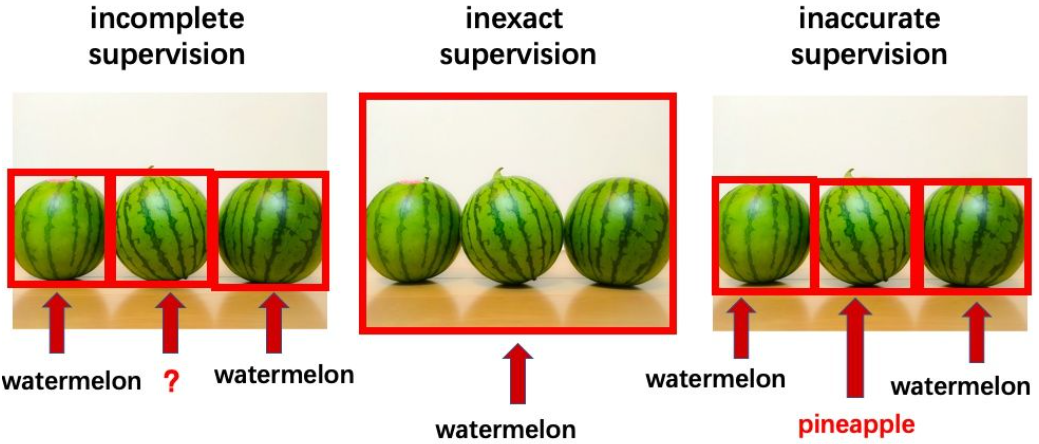
\includegraphics[width=0.8\linewidth]{images/weakly.png}
			\end{figure}
		\end{itemize}
	}
	\only<2>{
		\framesubtitle{{\normalsize Great performance of Event Camera}}
		\begin{figure}
			\centering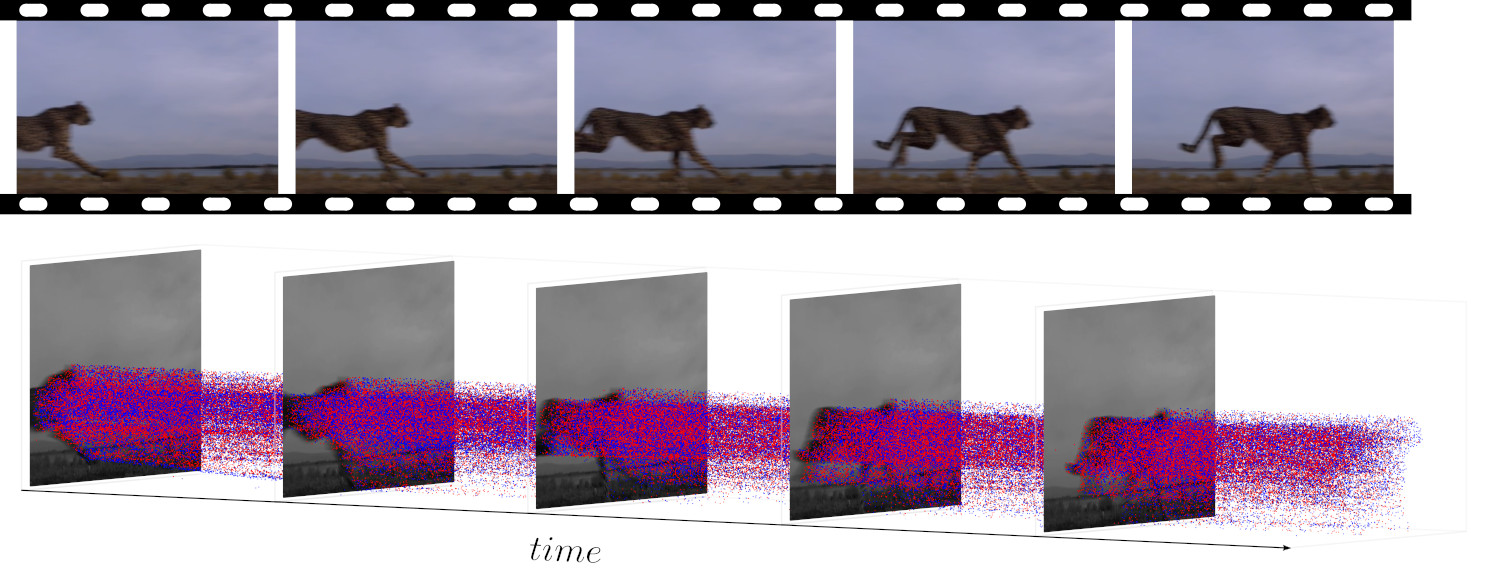
\includegraphics[width=0.85\linewidth]{images/Event_camera_comparison.jpg}
		\end{figure}
		\begin{itemize}
			\item High temporal resolution(microsecs)
			\item Low Latency
			\item Low Power(SNN, neuromorphic chip)
			\item No motion blur
			\item High dynamic range
		\end{itemize}
	}
	\end{frame}
	
	\begin{frame}{Motivation}
		\begin{itemize}
			\item Parameterized \alert{motion model} falls into an ill-posed problem when input frames are \alert{sparse}.
			\item Event-based methods: learn \alert{frame residual}, can't solve \alert{low-texture surface}, always need high frame-rate auxilary videos.
			\begin{figure}
				\centering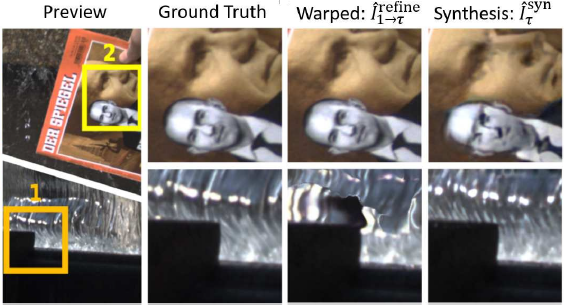
\includegraphics[width=0.7\linewidth]{images/warping_based_vs_event_based.png}
			\end{figure}
		\end{itemize}
	\end{frame}
	
	\begin{frame}{Contributions}
		\begin{itemize}
			\item Weakly supervised training, and perform SOTA, generalize well.
			\item Complementary appearance fusion\textit{(CAF)} for aggregates image and event appearance.
			\item Subpixel Motion Transformer\textit{(SMT)}, for super resolution\textit{(SR)} reconstruction.
			\item Contribute an event dataset, but not open source yet.
		\end{itemize}
	\end{frame}
	
	\begin{frame}{Proposed Method}
		\only<1>{
			\framesubtitle{Overview}
			\begin{figure}
				\centering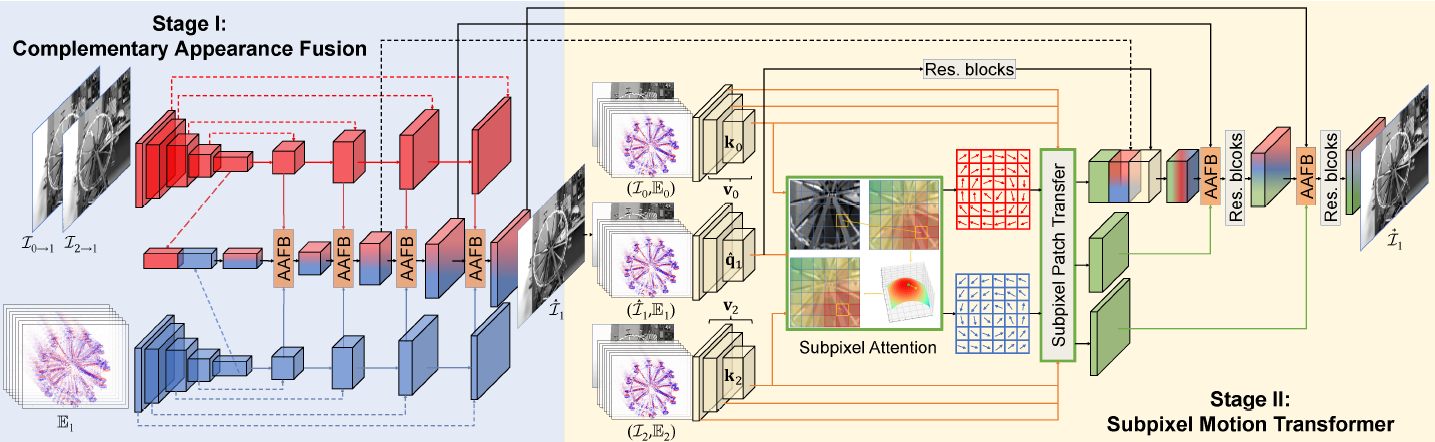
\includegraphics[width=0.95\linewidth]{images/overview.png}
			\end{figure}
			\begin{itemize}
				\item Two stages: complementary appearance fusion\textit{(CAF)} and subpixel motion transfer\textit{(SMT)}
				\item CAF stage: fuse images and events, get initial $ \hat{I_1} $.
				\item SMT stage: refine results with subpixel attention mechanism.
			\end{itemize}	
		}
		\only<2-5>{
			\framesubtitle{Stage \uppercase\expandafter{\romannumeral1}: Complementary appearance fusion(CAF)}
			\begin{figure}[htbp]
				\centering
				\begin{minipage}[t]{0.48\textwidth}
					\centering
					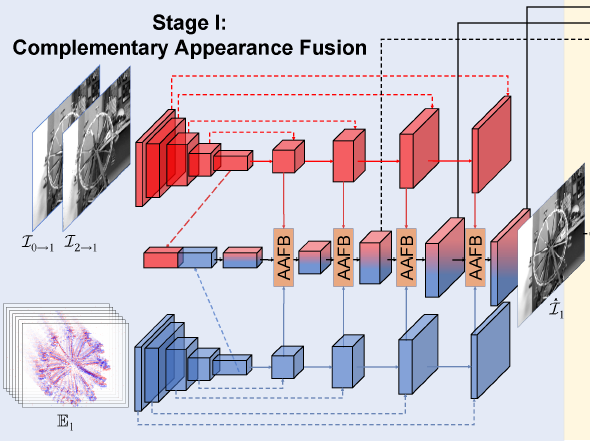
\includegraphics[width=5cm]{images/stage1.png}
					\caption*{Stage \uppercase\expandafter{\romannumeral1}}
				\end{minipage}
				\begin{minipage}[t]{0.48\textwidth}
					\centering
					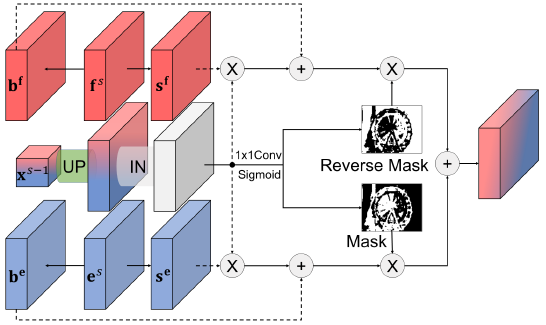
\includegraphics[width=6cm]{images/fusion.png}
					\caption*{AAFB}
				\end{minipage}
			\end{figure}
		}
		\only<2>{
			\begin{itemize}
				\item Prepare works:
				\begin{itemize}
					\item Forward warping $ \mathcal{I}_{0} $ and $ \mathcal{I}_{2} $ with PWC-Net\footfullcite{sun2018pwc} $ \to $ $\mathcal{I}_{0 \rightarrow 1},\ \mathcal{I}_{2 \rightarrow 1}$
					\item Event representation $ \mathbb{E}_{1} $
				\end{itemize}
			\end{itemize}
		}
		\only<3>{
			\begin{itemize}
				\item Adaptive Appearance Fusion Block(AAFB):
				\begin{equation}
					\mathbf{x}^{s}=g\left(\mathbf{x}_{\uparrow}^{s-1} ; \mathbf{f}^{s}, \mathbf{e}^{s}\right), s \in\{1,2,3,4,5\}
				\end{equation}
				$ \mathbf{x}_{\uparrow}^{s-1} $ denotes the $ 2\times $ upsampled version of $ \mathbf{x}^{s-1} $ \\
				$ \mathbf{f}^{s}, \mathbf{e}^{s} $ denotes 2 branches features.
			\end{itemize}
		}
		\only<4-5>{
			\begin{itemize}
				\item Adaptive Appearance Fusion Block(AAFB):
				\begin{equation}
					\mathbf{y}^{\mathbf{e}}=\left(\frac{\mathbf{x}_{\uparrow}^{s}-\mu\left(\mathbf{x}_{\uparrow}^{s}\right)}{\sigma\left(\mathbf{x}_{\uparrow}^{s}\right)}\right) \odot \mathbf{s}^{\mathbf{e}}+\mathbf{b}^{\mathbf{e}}
				\end{equation}
			\end{itemize}
		}
		\only<4>{
			\qquad Break up $ \mathbf{f}^{s},\ \mathbf{e}^{s} $ with scalings and biases $ \mathbf{s}^{\mathbf{f}} ,\ \mathbf{b}^{\mathbf{f}} $ and $ \mathbf{s}^{\mathbf{e}},\ \mathbf{b}^{\mathbf{e}} $
		}
		\only<5>{
			\begin{equation}
				y=y^{e} \odot \textbf{m}+y^{f}(1-\textbf{m})
			\end{equation}
		}
		\only<6>{
			\framesubtitle{Stage \uppercase\expandafter{\romannumeral2}: Subpixel Motion Transformer(SMT)}
			\begin{figure}
				\centering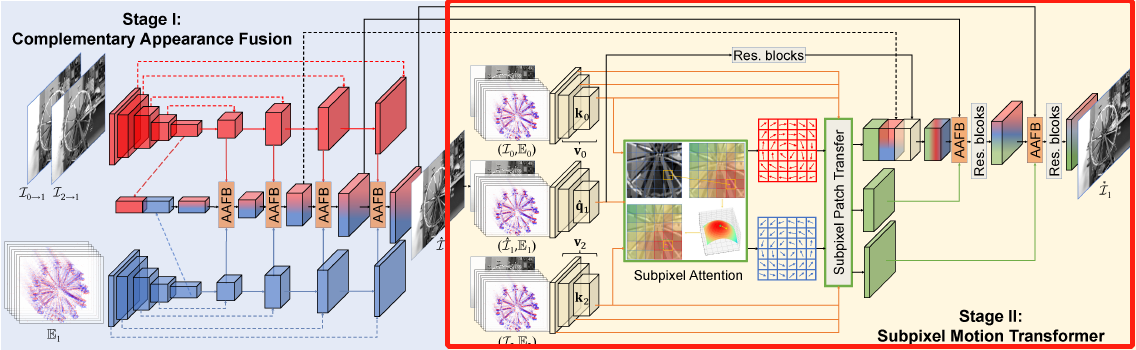
\includegraphics[width=0.95\linewidth]{images/subpixel.png}
			\end{figure}
		}
		\only<6>{
			\begin{itemize}
				\item Prepare works: \\
				\begin{itemize}
					\item $(\mathcal{I}, \mathbb{E})$ $ \xrightarrow[]{conv} $ $\left\{\mathbf{v}^{s} \mid s \in\{0,1,2\}\right\}$ as \alert{values}
					\item $ \mathbf{v}^2 $ $ \xrightarrow[]{clone} $ $ \mathbf{k}_{0},\ \mathbf{k}_{2} $ as \alert{keys}, $ \hat{\mathbf{k}}_{1} $ as \alert{query}
					\item relevance measure:
					\begin{equation}
						\mathbf{D}_{0}(\mathbf{i}, \mathbf{p})=\left\|\frac{\hat{\mathbf{k}}_{1}(\mathbf{i})}{\left\|\hat{\mathrm{k}}_{1}(\mathbf{i})\right\|_{2}}-\frac{\mathbf{k}_{0}(\mathbf{i}+\mathbf{p})}{\left\|\mathbf{k}_{0}(\mathbf{i}+\mathbf{p})\right\|_{2}}\right\|_{2}^{2}
					\end{equation}
					$\mathbf{p} \in[-m, m]^{2}$ represents a spatial \alert{offset}.
				\end{itemize}
			\end{itemize}
		}
		\only<7>{
			\framesubtitle{Stage \uppercase\expandafter{\romannumeral2}: Subpixel Motion Transformer(SMT)}
			\begin{figure}
				\centering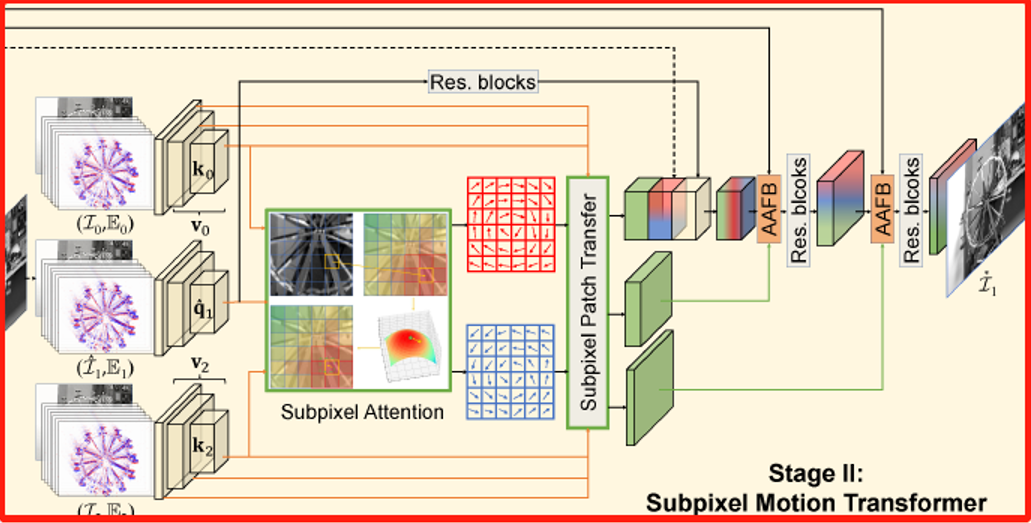
\includegraphics[width=0.5\linewidth]{images/subpixel2.png}
			\end{figure}
			\begin{itemize}
				\item Subpixel attention learning: \\
				\begin{equation}
					\mathrm{j}=\mathrm{i}+\mathrm{p}^{*} \text { where } \mathrm{p}^{*}=\arg \min _{\mathrm{p}} \mathrm{D}_{0}(\mathrm{i}, \mathrm{p})
				\end{equation}
				\begin{equation}
					\mathbf{d}(\mathbf{u})=\mathbf{D}_{0}\left(\mathbf{i}, \mathbf{p}^{*}+\mathbf{u}\right), \mathbf{u} \in \mathbb{Z}^{2} \cap[-n, n]^{2}
				\end{equation}
				\begin{equation}
					\mathrm{d}(\mathbf{u}) \approx \hat{\mathrm{d}}(\mathbf{u})=\frac{1}{2} \mathbf{u}^{\mathrm{T}} \mathbf{A} \mathbf{u}+\mathbf{b}^{\mathrm{T}} \mathbf{u}+c
				\end{equation}
				\begin{equation}
					\min _{\mathbf{A}, \mathbf{b}, c} \sum_{\mathbf{u}} \mathrm{w}(\mathbf{u})\|\hat{\mathbf{d}}(\mathbf{u})-\mathrm{d}(\mathbf{u})\|^{2}
				\end{equation}
			\end{itemize}
		}
		\only<8>{
			\framesubtitle{Stage \uppercase\expandafter{\romannumeral2}: Subpixel Motion Transformer(SMT)}
			\begin{figure}
				\centering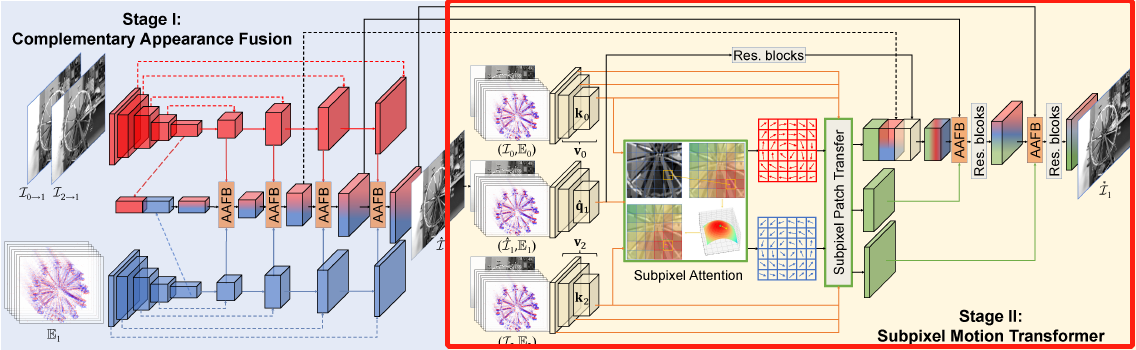
\includegraphics[width=0.95\linewidth]{images/subpixel.png}
			\end{figure}
			\begin{itemize}
				\item Subpixel patch transfer:
				\begin{itemize}
					\item distance means relevalce($ K \cdot Q$), then mutiply with $ V $, get transferred values $\mathbf{z}_{0}^{s}$ and $\mathbf{z}_{2}^{s}$
					\item select transferred values
					\begin{equation}
						\mathrm{z}_{1}^{s}(\mathrm{i})=\left\{\begin{array}{l}
							\mathrm{z}_{0}^{s}(\mathrm{i}), \text { if } \mathrm{D}_{0}\left(\mathrm{i}, \mathrm{p}_{0}^{*}\right)<\mathrm{D}_{2}\left(\mathrm{i}, \mathrm{p}_{2}^{*}\right) \\
							\mathrm{z}_{2}^{s}(\mathrm{i}), \text { otherwise. }
						\end{array}\right.
					\end{equation}
					\item fuse with previous features
				\end{itemize}
			\end{itemize}
		}	
		\only<9>{
			\begin{figure}
				\centering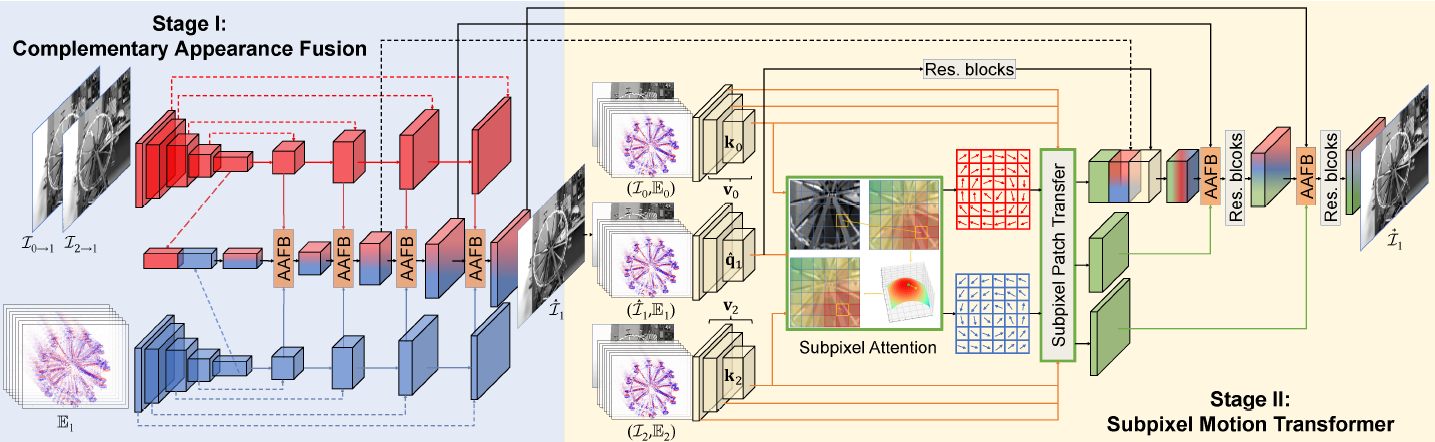
\includegraphics[width=0.95\linewidth]{images/overview.png}
			\end{figure}
			\begin{itemize}
				\item Settings:
				\begin{itemize}
					\item Datasets: GroPro(720p, 240FPS), SloMo-DVS dataset(self-collected) \\
					Adopt \alert{$ 10\times $}, so sample 1th, 11th, 21th frames to form a \alert{sparse} training triplet to train.
					\item Loss: Charbonnier Loss(superior to $ \ell_1,\ \ell_2 $ loss)
					\begin{equation}
						\text { Charbonnier\_loss }=\sqrt{x^{2}+\epsilon^{2}}
					\end{equation}
				\end{itemize}
			\end{itemize}
		}
		\only<10>{
			\framesubtitle{Thoughts}
			\begin{figure}
				\centering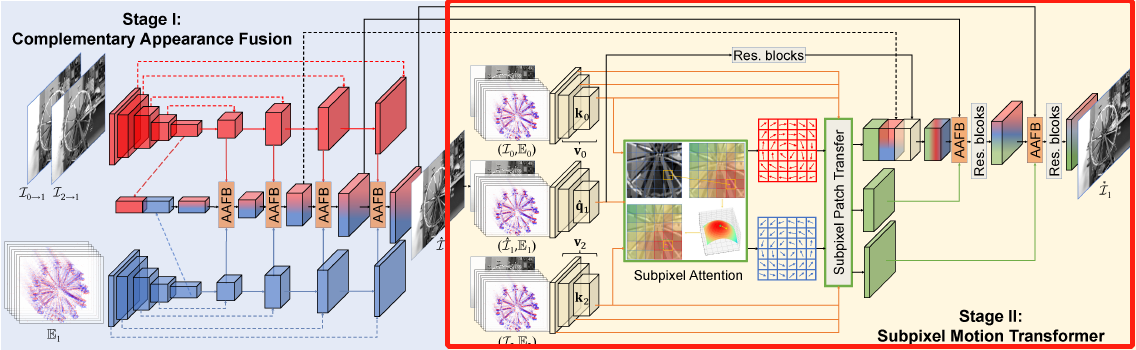
\includegraphics[width=0.95\linewidth]{images/subpixel.png}
			\end{figure}
			\begin{itemize}
				\item Frame info still rely on optical flow, not end-to-end.
				\item Process event in image format, point cloud or 3D conv works?
				\item 240FPS with sample rate 10 $ \xLongleftrightarrow{versus} $ 25FPS with sample rate 1, which is weakly supervision?
			\end{itemize}
		}
	\end{frame}


	\begin{frame}{Experiments}
		\framesubtitle{Quatitative results}
			\begin{figure}
				\centering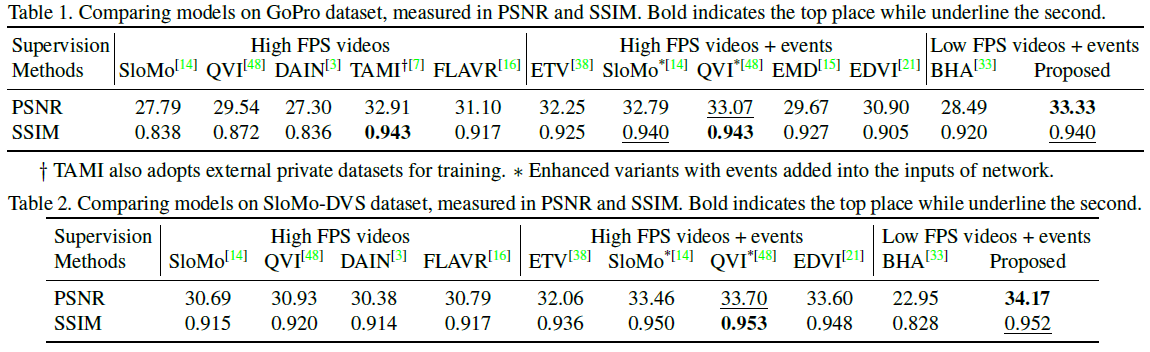
\includegraphics[width=0.95\linewidth]{images/result1.png}
			\end{figure}
	\end{frame}

	\begin{frame}{Experiments}
		\framesubtitle{Abalation Study}
		\begin{figure}
			\centering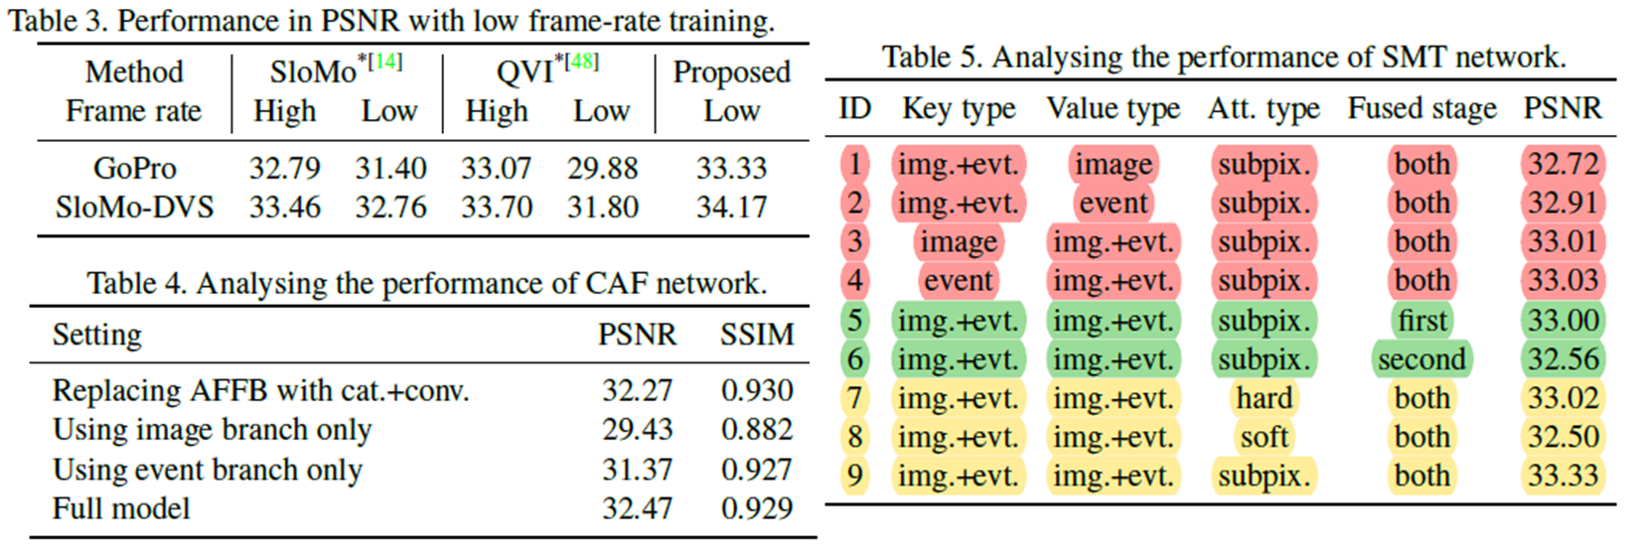
\includegraphics[width=0.95\linewidth]{images/result2.png}
		\end{figure}
	\end{frame}

	\begin{frame}{Experiments}
		\framesubtitle{Qualitative results}
		\begin{figure}
			\centering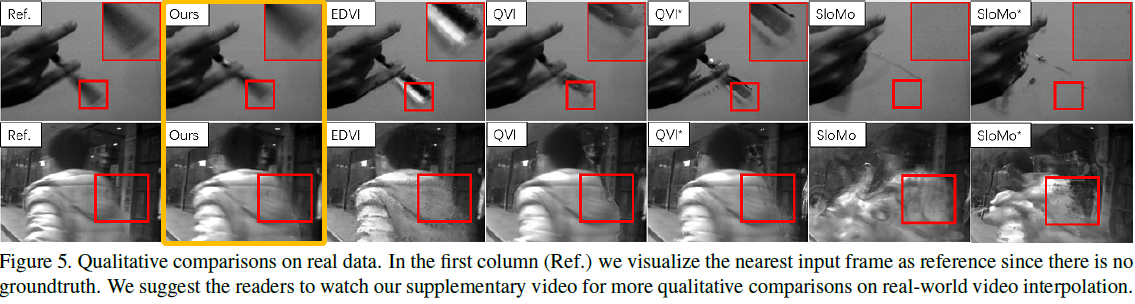
\includegraphics[width=0.95\linewidth]{images/result3.png}
		\end{figure}
	\end{frame}

	\begin{frame}{Experiments}
		\framesubtitle{Qualitative results}
		\begin{figure}
			\centering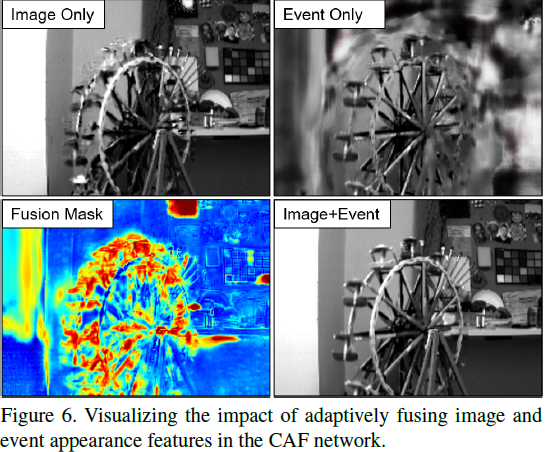
\includegraphics[width=0.6\linewidth]{images/result4.png}
		\end{figure}
	\end{frame}

	\begin{frame}{Experiments}
		\framesubtitle{Qualitative results}
		\begin{figure}
			\centering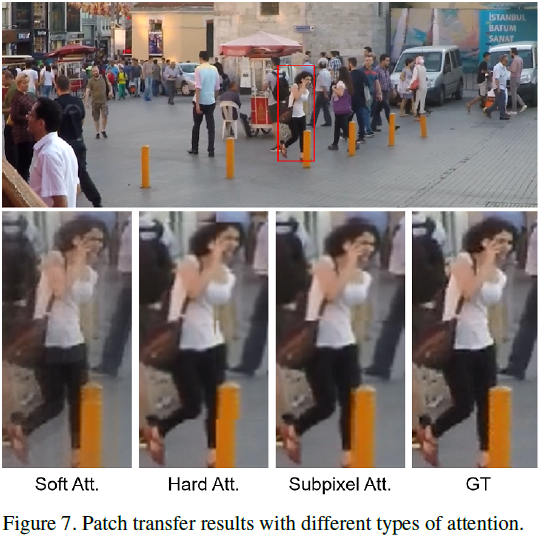
\includegraphics[width=0.6\linewidth]{images/result5.png}
		\end{figure}
	\end{frame}

	\begin{frame}{Conclusions}
		\begin{figure}
			\centering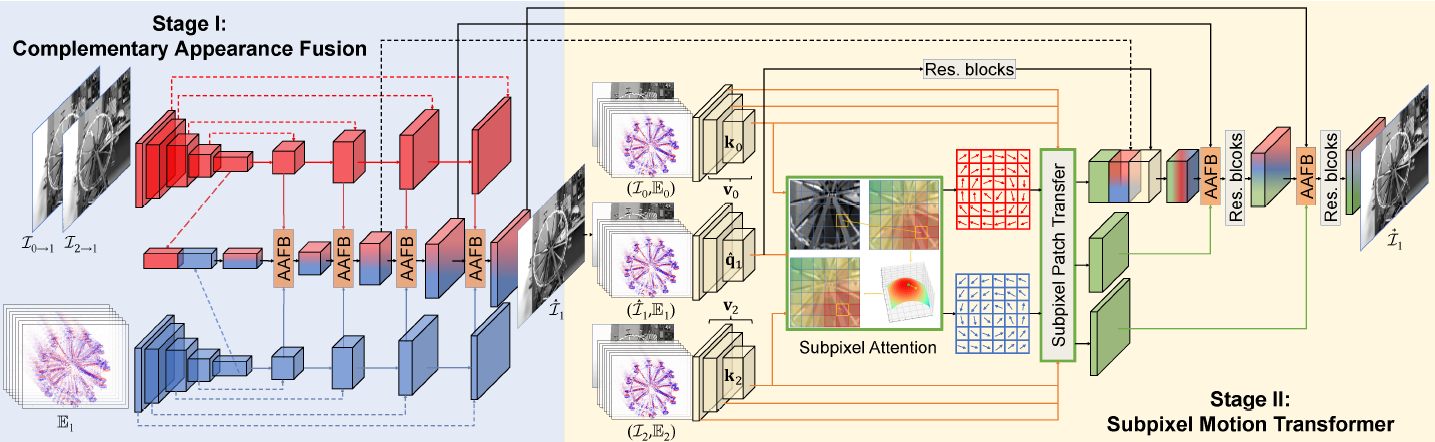
\includegraphics[width=0.95\linewidth]{images/overview.png}
		\end{figure}
		\begin{itemize}
			\item Train with low frame-rate videos, but outperform others and generalize well.
			\item Attention mechanism, no direct motion modelling, eg optical flow.
		\end{itemize}
	\end{frame}

	\begin{frame}{}
		\centering \Huge
		\emph{Thanks,  Q \& A }
	\end{frame}
\end{document}
